\documentclass[letterpaper, 12pt]{article}
\usepackage[letterpaper, top=2.5cm, bottom=2.5cm, left=3cm, right=3cm]{geometry} %margenes
\usepackage[backend=biber]{biblatex}\addbibresource{referencias.bib}
\usepackage[utf8]{inputenc} %manejo de caracteres especiales
\usepackage[spanish]{babel} %manejo de encabezados de inglés a español
\usepackage{fancyhdr} %formato de los encabezados de página
\usepackage{ragged2e} %alineado real justficado
\usepackage{graphicx} %manejo de imagenes
\usepackage{amsmath} %manejo de notación matemática
\usepackage{mathtools} %manejo de notación matemática
\usepackage{blindtext} %texto de relleno
\usepackage{tikz} %manejo de diagramas electricos
\usepackage{circuitikz} %manejo de diagramas electricos
\usepackage{csquotes}
\usepackage[titles]{tocloft} %manejo de elementos para el índice
\usepackage{float} %manejo de centrado para figuras

\pagestyle{fancy}
\fancyhf{}
\rfoot{\thepage}

\nocite{*}

\begin{document}
    
    %PORTADA
    \begin{titlepage}
        \begin{figure}[ht]
            \centering
            
\includegraphics[width=15cm]{logosITT.png}
        \end{figure}
        \centering
        {\scshape\LARGE Tecnológico Nacional de México\\Instituto Tecnológico de Tijuana\par}
        \vspace{1cm}
        {\scshape\Large Princípios Electricos y Aplicaciones Digitales\par}
        \vspace{1cm}
        {\scshape\Large Unidad 1\par}
        \vspace{1.5cm}
        {\huge\bfseries Tarea 3\par}
        \vspace{2cm}
        {\Large\itshape Equipo D1N4Mic B00M\par}
        \vfill
        Profesor: \par
        Ing. Rigoberto Alvarado Rivera
        
        \vfill

        {\large 11 de diciembre del 2020}
    \end{titlepage}

    \newpage
    \thispagestyle{empty}
    \tableofcontents
    \listoffigures

    \newpage
    \setcounter{page}{1}
    \thispagestyle{fancy}
    \lhead{\textbf{Tarea 3}}
    \rhead{\text{18 de diciembre del 2020}}
    \section{Diferencias entre una computadora de 64 bits y de 32 bits}
    \begin{itemize}
        \item Las computadora de 64 bits soportan más RAM comparado a las de 32 bits.
        \item Los programas diseñados para 64 bits procesan más rapido comparado a los de 32 bits.
        \item Las computadoras de 64 bits soportan OS de 64 y 32 bits.
        \item Los OS de 64 bits son retrocompatibles con las tarjetas gráficas.
        \item En 64 bits (por el soporte de RAM) los programas optimizados para multi-tareas son más rápidos.
    \end{itemize}
    \section{Conclusión: mejor sistema que ofrece una mejor calidad de sonido (vinilo analógico contra formato digital)}
    \justify
    El sistema que ofrece la mejor calidad es el vinilo analógico. Como se ha visto a lo largo de la materia, los sistemas analógicos son lo que capturan de la manera más fiel
    el entorno comparado al digital, que éste comprime las señales a rangos de ceros y unos, lo cual no es fiel a la realidad inmediata. Pero la diferencia sonora es bastante imperceptible para el escucha promedio
    al momento de comparar ambos formatos.
    \section{Principio de funcionamiento de pantallas LCD, LED y OLED}
    \justify
    Se explica los principios de funcionamiento de las distintas tecnologías de pantallas modernas.
    \subsection{LCD}
    \justify
    Por sus siglas en inglés \emph{Liquid Crystal Display} se define por el mismo nombre de su tecnología. Es una combinación de los estados sólidos y líquidos donde dichos cristales se usan para
    producir una imágen visible. Su principio básico es el de bloquear luz en vez de emitirla. Estos requieren una luz trasera ya que estos mismos no la emiten. Cuando una corriente se le aplica al LCD
    las moleculas del material se desenvuelven causando que el ángulo de la luz que pasa por la molecula y el cambio en el ángulo del filtro dando como resultado que un poco de luz pase del vidrio polarizado
    a un área específica del LCD. 
    \begin{figure}[H]
        \centering
        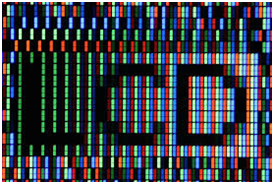
\includegraphics[width=10cm]{LCD.png}
        \caption{Ejemplo físico de un LCD.}
    \end{figure} 
    \subsection{LED}
    \justify
    Por sus siglas en inglés \emph{Light Emitting Diode} se define como un componente eléctrico que emite luz cuando por este fluye una corriente. El principio de funcionamiento se deriva de su clasificación como
    semiconductor PN. Cuando el electrón libre está en movimiento, existe un cambio del nivel de energía al momento de que el voltaje baja de la banda de conducción. Esto causa una descarga de energía por el movimento del electrón y debido
    a que este diodo expresa dicha descarga como luz, permite que este exprese la iluminación.
    \begin{figure}[H]
        \centering
        
\includegraphics[width=10cm]{LED.png}
        \caption{Símbolo del LED.}
    \end{figure}
    \subsection{OLED}
    \justify
    La tecnología OLED trabaja principalmente con un emitidor de las mismas siglas - este emitidor es un material organico (a base de carbono) que emiten luz cuando se le aplica electricidad. Esto es debido a las capas usadas:
    \begin{itemize}
        \item Cátodo.
        \item Capa Transportadora de Electrones (ETL).
        \item Capa de Bloqueo (RL).
        \item Capa Emisiva.
        \item Capa con orificios Transportadora. (HTL).
        \item Capa con orificios inyectora (HIL).
        \item Anodo.
        \item Sustrato.
    \end{itemize}
    A continuación se muestra una imágen que ilustra dichas capas.
    \begin{figure}[H]
        \centering
        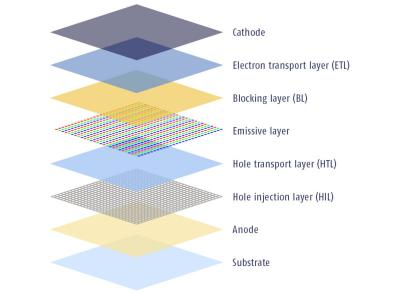
\includegraphics[width=10cm]{OLED.jpg}
        \caption{Estructura del dispositivo OLED.}
    \end{figure}
    \section{Relación de la calidad de imágen con la cantidad de pixeles de una cámara digital}
    \justify
    Están estrechamente relacionado al momento en el cual la imágen se tomaron. Esto es debido a la cantidad de pixeles por pulgada, la relación es simple ya que a mayores pixeles por pulgada, mayór es la resolución porque dichos pixeles son usados para procesar más o menos detalles
    dependiendo de dichos PPI (\emph{Pixels per inch}). Dependiendo de los factores externos como la iluminación del lugar de la foto influyen en la calidad de imágen.
    \begin{figure}[H]
        \centering
        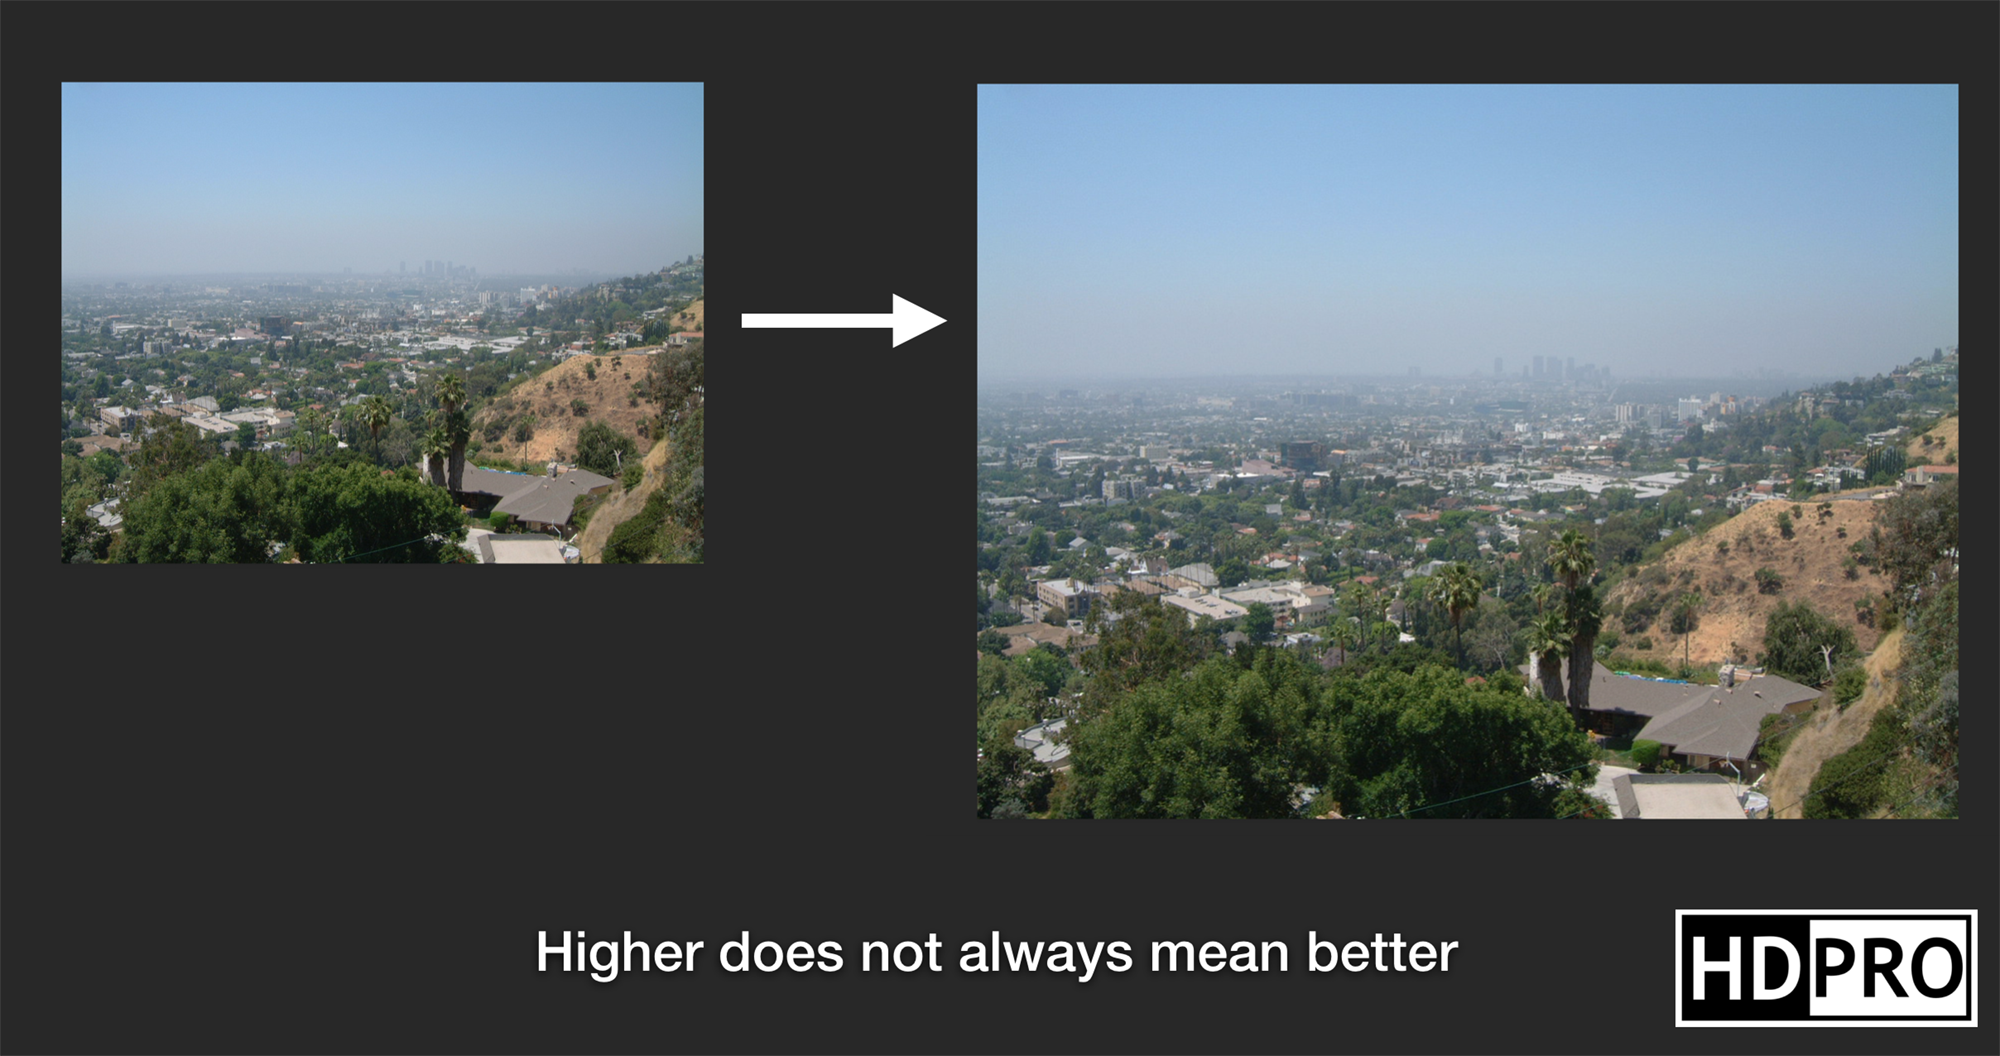
\includegraphics[width=10cm]{higlow.png}
        \caption{Comparación de calidad de una foto.}
    \end{figure}
    \section{Necesidad de protocolos de compresión de audio y video}
    \justify
    La razón es muy sencilla, comprimir archivos permite reducir el tamaño del archivo y así poder ser almacenados o transferidos de manera más sencilla. Esto es porque un menor tamaño de un archivo permite que este sea transferido en un menor tiempo (dependiendo la velocidad de la red).
    \section{Protocolos de compresión de video de Facebook, Twitter e Instagram}
    \justify
    El protocolo común de compresión para dichas aplicaciones es el H.264; este consiste en un estándar de video de baja calidad de videocoferencias y aplicaciones de internet, basado en 8bits/muestra. Su intención principal de crear dicho estándar capaz de proporcionar una buena calidad de imagen
    con tasas binarias notablemente inferiores a los estándares previos y no incrementar la complejidad de su diseño.
    \newpage
    \thispagestyle{empty}
    \addcontentsline{toc}{section}{Referencias}
    \printbibliography

\end{document}